\section{Background}
\begin{figure}[t!]
  \centering
  % Requires \usepackage{graphicx}
  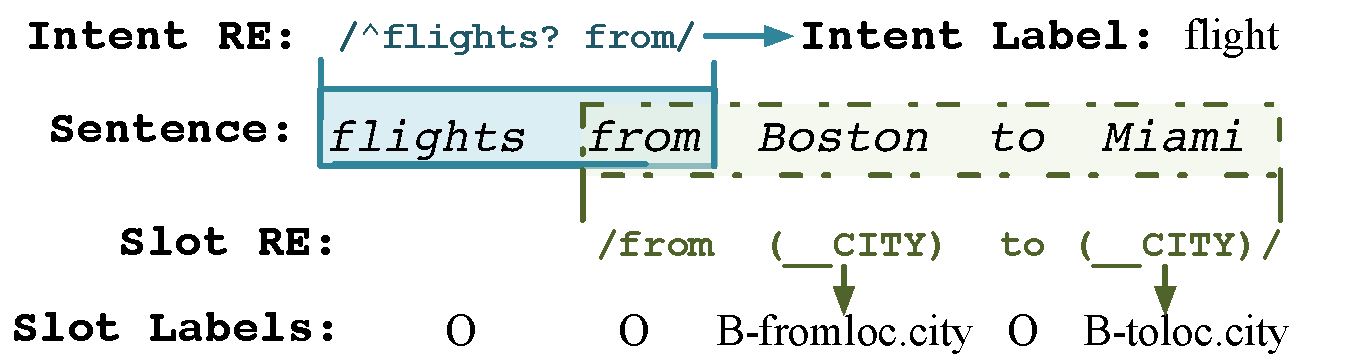
\includegraphics[width=0.5\textwidth]{figure/motivation.pdf}\\
  \caption{An example sentence from the ATIS corpus. \REs can be used to detect the intention and label slots.}\label{atis_sample}
\end{figure}

\subsection{Problem Definition}
While our approach is generally applicable, to evaluate our approach on concrete and measurable objectives, we target two areas of spoken
language understanding: \emph{intention detection} and \emph{slot filling}. The former is a sentence classification task where we learn a
function to map an input sentence of $n$ words, $\textbf{x}=[x_{1}, ..., x_{n}]$, to a corresponding intention, $c$. The latter is a
sequence labeling task for which we learn a function to map an input query sentence of $n$ words, $\textbf{x}=[x_{1}, ..., x_{n}]$, to a
corresponding labeling sequence, $\textbf{y}=[y_{1}, ..., y_{n}]$, where each element, $y_i$, is the slot label of the corresponding word,
$x_i$,  of the input query.


%Intent detection is a typical sentence classification task.
%We need to learn a mapping function that maps an input sentence $\textbf{x}$, where $\textbf{x}=[x_{1}, ..., x_{n}]$ is the input sentence with $n$ words, to the corresponding intent $y$.
%% $f: \mathcal{X} \rightarrow \mathcal{Y}$
%% Given a set of training examples $\{(x_i, y_i): i=1,...,N\}$,
%
%On the other side, slot filling is often treated as a sequence labeling task.
%We need to learn a mapping function that maps an input query sentence $\textbf{x}$ to the corresponding label sequence $\textbf{y}$, where $\textbf{y}=[y_{1}, ..., y_{n}]$ is the slot labels of each word.
% Here we also have a set of training examples $\{(\textbf{x}_i, \textbf{y}_i): i=1,...,N\}$, where $\textbf{x}_i=[x_{i1}, ..., x_{in_i}]$ is the input sentence with $n_i$ words, and $\textbf{y}_i=[y_{i1}, ..., y_{in_i}]$ is the slot label of each word.

%For example, Figure\ref{atis_sample} shows a sample sentence in the ATIS dataset. Its intent is \emph{flight}, indicating the user wants
%flight-related information. We also need to identify the \emph{from\_city} and the \emph{to\_city} slots so that the we can return the
%correct information.

\cparagraph{Example} Figure \ref{atis_sample} gives an example query sentence from the ATIS dataset\todo{\cite{}}. A successful intention
detection would suggest the intention of the sentence is \emph{flight}, i.e., the query is about flight-related information. Slot filling,
on the other hand, would need to identify the \emph{from\_city} and \emph{to\_city} slots by correctly labeling the sentence using e.g.,
the standard begin-inside-outside (\texttt{BIO}) scheme.




%\begin{table}
%\setlength{\tabcolsep}{0.23em}
%\centering
%\small{
%\begin{tabular}{ll}
%
%\toprule
%\textbf{Sentence} &flights \;\;\;\;\;\;\;\; from \;\;\;\; boston \;\;\;\;\; to \;\;\; miami  \\
%\midrule
%\textbf{Intent \RE} & \multicolumn{1}{l}{/\textasciicircum \texttt{flights?} \texttt{from}/} \\
%\textbf{Intent} &\multicolumn{1}{l}{\emph{flight}} \\
%\textbf{Slot \RE} & \multicolumn{1}{l}{\quad\quad\quad\;\;\;\;\;\;/\texttt{from} \; \texttt{(\_\_CITY)} \, \texttt{to}  \texttt{(\_\_CITY)}/} \\
%\textbf{Slot Label} &\;\;\; \emph{O} \;\;\;\;\;\;\;\;\;\;\; \emph{O} \; \emph{B-fromloc.city} \, \emph{O} \, \emph{B-toloc.city} \\
%\bottomrule
%\end{tabular}
%}
%\caption{A sample sentence from ATIS corpus, with intent, slot and example \RE patterns.}
%\label{atis_sample}
%\end{table}


\subsection{The Use of Regular Expressions}
\label{re_desc}

Our approach uses \REs to capture expert knowledge. Specifically, a \RE defines the mapping from a \emph{pattern} to an intention or a slot
labeling sequence. A search function takes in a \RE, applying it to a sentence, and returning all texts that match the pattern. The
matching results will then associated with an intention or a slot labeling sequence. The search is designed to return every match on a
sentence (\z{or just return the first match?}).

We give each target intention and slot a label, which we respectively refer as an \emph{\textbf{intention label}} and a \emph{\textbf{slot
label}}. The outcome of applying a \RE to a sentence can be an intention or a slot labeling sequence -- if there exists a pattern match. We
call the matching outcome a \emph{\textbf{REtag}}.
%We denote the output of \RE as \textbf{\emph{\RE tag}}, and the label
%that we want to predict as \textbf{\emph{intent label}} and \textbf{\emph{slot label}} for intent detection and slot filling respectively,
%which are generally referred to as \textbf{\emph{target label}}.
Note that, while not necessarily the same as the target label, a \REtag is usually related to one or more target labels. For example, a
\REtag \emph{CITY} is related to: \emph{fromloc.city}, \emph{toloc.city}, \emph{stoploc.city}. \z{The last sentence is confusing, please
rephrase. Please also check if a \REtag can be mapped to a slot labeling sequence. After reading the description of slotting filling, it
looks like we can use part of the \RE for evaluation.}

In this work, the \REtag for intention detection is a pre-defined intention label. For example, an \RE of \texttt{/\textasciicircum
flights?\:from/} can be associated with an intention label \emph{flight}; and when applying this \RE to the sentence given in
Figure~\ref{atis_sample} for intention detection, we get a \REtag of \emph{flight}.

For slot filling, we use two different sets of \texttt{RE}s. Given the group functionality of \RE, we can assign tags to our interested
\textbf{\emph{\RE groups}} (the text surrounded by brackets). (1)~For the method in Sec.~\ref{interact_with_module}, since we need to
annotate clue words for certain slot labels, its \RE tag is the same as the slot labels. For example, \texttt{/(from)\:(\_\_CITY)/} will
match the sentence in Figure~\ref{atis_sample}, and assign \emph{fromloc.city} to the second \RE group. Here \emph{\_\_CITY} is a list of
all the city names, which can be repalced with a string like \texttt{/boston|miami|LA/}. Note that, an ordinary word list pattern can be
written as strings like \texttt{/(\_\_CITY)/} in \RE. (2)~For the methods in Sec.~\ref{fusion_with_input} and \ref{fusion_with_output}, the
\RE tag is different from the slot label. For example, the second \RE group in \texttt{/(from)\:(\_\_CITY)/} will be tagged as \emph{city},
which is a simplified version of the slot label. The reason that we use different \texttt{RE}s here is to give an example that \texttt{RE}s
with output different from the target labels can also make improvements to \NN.

% We use another set of \texttt{RE}s for the methods in Sec.~\ref{fusion_with_input} and \ref{fusion_with_output} because using simpler tags can significantly reduce the complexity of the \RE, and therefore making the generation of \RE much easier. For example, we need \texttt{/(from)\:(\_\_CITY)/} to identify \emph{fromloc.city}, but only \texttt{/(\_\_CITY)/} to identify \emph{city}.

When writing \RE patterns, since complicated \texttt{RE}s often lead to better performance but require more efforts to generate, \RE complexity is usually an important trade-off that we need to make. Generally, two aspects of \RE influence the complexity most. First, \RE complexity increases with the number of \RE groups. This kind of complexity will lead to better precision and lower coverage. Second, \RE complexity also increases with the number of \emph{or}s (the symbol $|$) in an \RE group. Here a group can be considered as a set of phrases that express the same meaning. Therefore, this kind of complexity usually results in higher coverage and slightly lower precision.
% unless adding ambiguous phrases to the group

% Note that, while the outputs are the intent or slot themselves in the examples above, the \RE output can also be a tag related to, but not the same as, the label that we want to predict.
% We allow this variation because using tags different from the target labels can sometimes make it easier to write an \RE. For example, we need \texttt{/from\:(\_\_CITY)/} to identify \emph{fromloc.city}, but only \texttt{/(\_\_CITY)/} to identify \emph{city}. In this paper, the output of intent patterns is the same as the intent label, and the output of slot patterns used by the method in Section \ref{interact_with_module} is the same as the slot label. However, the slot \RE tag for methods in Section \ref{fusion_with_input} and \ref{fusion_with_output} is the entity part of the slot label (e.g., \emph{city} in \emph{fromloc.city}).
